% ============================================================================
% Multi-Component Loss Balancing for Deep Learning
% Duration: 30 minutes, after lunch on Day 1
% ============================================================================

\documentclass[aspectratio=169,11pt]{beamer}

% ---------- Theme and colors ----------
\usecolortheme{dove}
\setbeamertemplate{navigation symbols}{}
\setbeamertemplate{footline}{%
  \hfill\usebeamerfont{page number in head/foot}%
  \usebeamercolor[fg]{normal text}%
  \insertframenumber\,/\,\inserttotalframenumber\kern1em\vskip4pt}
\setbeamerfont{frametitle}{size=\huge}

% ---------- Packages ----------
\usepackage[utf8]{inputenc}
\usepackage[T1]{fontenc}
\usepackage{amsmath,amssymb,amsfonts}
\usepackage{bm}
\usepackage{graphicx}
\usepackage{tikz}
\usetikzlibrary{shapes,arrows.meta,positioning,calc,fit,backgrounds,patterns,decorations.pathreplacing}
\usepackage{pgfplots}
\pgfplotsset{compat=1.18}
\usepackage{booktabs}
\usepackage{hyperref}
\usepackage{multicol}
\usepackage{xcolor}
\usepackage{algorithm}
\usepackage{algorithmic}

% ---------- Custom colors ----------
\definecolor{uzhblue}{rgb}{0,0,0.5}
\definecolor{uzhgreylight}{RGB}{236,238,241}
\definecolor{uzhgreydark}{RGB}{81,86,94}
\definecolor{harvardcrimson}{RGB}{153,0,0}
\definecolor{unil@blue}{RGB}{0,140,204}
\definecolor{unil@black}{RGB}{35,31,32}
\definecolor{darkgreen}{RGB}{0,100,0}
\definecolor{darkred}{RGB}{139,0,0}
\definecolor{softblue}{RGB}{70,130,180}
\definecolor{softorange}{RGB}{230,159,0}
\definecolor{softgreen}{RGB}{0,158,115}

% ---------- Set beamer colors ----------
\setbeamercolor{frametitle}{bg=uzhgreylight, fg=uzhblue}
\setbeamercolor{title}{fg=uzhblue}
\setbeamercolor{structure}{fg=uzhblue}
\setbeamercolor{block title}{bg=unil@blue, fg=white}
\setbeamercolor{block body}{bg=uzhgreylight}
\setbeamercolor{block title alerted}{bg=darkred,fg=white}
\setbeamercolor{block body alerted}{bg=red!5}
\setbeamercolor{block title example}{bg=darkgreen,fg=white}
\setbeamercolor{block body example}{bg=green!5}
\setbeamercolor{item}{fg=unil@black}
\setbeamercolor{normal text}{fg=unil@black}

% ---------- Emphasis and hyperlinks ----------
\newcommand{\emphc}[1]{\textcolor{harvardcrimson}{#1}}
\hypersetup{colorlinks,linkcolor=harvardcrimson,urlcolor=harvardcrimson}

% ---------- Math commands ----------
\newcommand{\x}{\bm{x}}
\newcommand{\w}{\bm{w}}
\newcommand{\bb}{\bm{b}}
\newcommand{\z}{\bm{z}}
\newcommand{\W}{\bm{W}}
\newcommand{\X}{\bm{X}}
\renewcommand{\a}{\bm{a}}
\newcommand{\R}{\mathbb{R}}
\newcommand{\E}[1]{\mathbb{E}\!\left[#1\right]}
\DeclareMathOperator*{\argmin}{arg\,min}
\DeclareMathOperator*{\argmax}{arg\,max}

% ---------- Title ----------
\title[Loss balancing -- Padova 2026]%
{Deep Learning for Solving Dynamic Models}
\subtitle{Session 3b: Loss balancing for multi-component residuals}
\author{Simon Scheidegger}
\institute[HEC Lausanne]{HEC, University of Lausanne}
\date{University of Padova\\September 23, 2026}

\begin{document}
% --- Exercise pause badge ---
\newcommand{\exercisepause}{%
  \tikz[baseline=(X.base)]{\node[fill=darkgreen!80!black, text=white,
  rounded corners=2pt, inner sep=3pt, font=\scriptsize\bfseries](X){PAUSE, 5 min};}}


% ============================================================================
% TITLE
% ============================================================================

% --- Slide 1: Title ---
{\setbeamercolor{background canvas}{bg=uzhgreylight}
\begin{frame}
\titlepage
\end{frame}
}

% --- Slide 2: Roadmap ---
\begin{frame}{Roadmap of This Lecture}
\begin{columns}[T]
\column{0.48\textwidth}
\textbf{I. Motivation}
\begin{itemize}
    \item Multi-component losses in PINNs and DEQNs
    \item The scale problem, and what it does to the gradient
\end{itemize}

\vspace{0.2em}
\textbf{II. Balancing Methods}
\begin{itemize}
    \item Equal weighting
    \item \textbf{Natural units} (the fix to do first)
    \item Inverse-loss weighting (+ finger exercise)
    \item SoftAdapt, \textbf{ReLoBRaLo}, GradNorm
\end{itemize}

\column{0.48\textwidth}
\textbf{III. Experiments \& Wrap-up}
\begin{itemize}
    \item Setup and results, three seeds
    \item Sensitivity to temperature $T$
    \item The same measurement on a DEQN
    \item Connection to PINNs \& DSGE
    \item Summary and references
\end{itemize}
\end{columns}

\vspace{-0.3em}
\begin{center}
{\scriptsize Hands-on: \texttt{03\_03\_Loss\_Normalization.ipynb} in \texttt{day1/code/03\_nas\_loss\_balancing/}}
\end{center}
\end{frame}

% --- Learning objectives ---
\begin{frame}{Learning objectives}
\textbf{By the end of this lecture you should be able to:}
\begin{itemize}
  \item Measure gradient dominance: record the gradient norm each weighted loss component sends to the shared parameters
  \item Write equilibrium residuals in natural units before any weighting rule is applied, and say why this comes first
  \item Implement inverse-loss weighting and ReLoBRaLo in a few lines, and state what each one balances: levels, or progress
  \item Read a loss-balancing result as a median over seeds with its range, on a scale-free error
  \item Tell a transient scale gap from a permanent one on a DEQN, using the gradient-norm ratio after the transient
\end{itemize}
\end{frame}


% ============================================================================
% PART 1: MOTIVATION
% ============================================================================

% --- Slide 3: Part I Divider ---
\begin{frame}[plain,c]
\begin{center}
{\Huge \textcolor{uzhblue}{\textbf{Part I}}}\\[12pt]
{\LARGE Motivation}
\end{center}
\end{frame}

% --- Slide 4: Motivation ---
\begin{frame}{Motivation: Multi-Component Losses}
\textbf{Many problems in economics require minimizing \emph{several} loss terms simultaneously:}

\vspace{0.3cm}
\begin{columns}[T]
\column{0.50\textwidth}
\textbf{Physics-informed NNs (PINNs):}
\begin{itemize}
    \item PDE residual $\mathcal{L}_\text{PDE}$
    \item Boundary conditions $\mathcal{L}_\text{BC}$
    \item Initial conditions $\mathcal{L}_\text{IC}$
\end{itemize}

\vspace{0.3cm}
\textbf{Deep equilibrium nets (DEQNs):}
\begin{itemize}
    \item Euler equation residuals
    \item Budget constraints
    \item Market clearing
\end{itemize}

\column{0.47\textwidth}
\textbf{Multi-task learning:}
\begin{itemize}
    \item Predict multiple outputs from shared features
    \item Each output has its own loss
\end{itemize}

\vspace{0.3cm}
\begin{alertblock}{Core challenge}
These loss components often live at \emphc{vastly different scales}.
\end{alertblock}
\end{columns}
\end{frame}

% --- Slide 3: The Scale Problem ---
\begin{frame}{The Scale Problem}
\begin{columns}[T]
\column{0.50\textwidth}
\textbf{Example:} three targets of the same shape complexity, at scales $1$, $10^2$, $10^4$. Squared errors then sit at
\begin{align*}
    \mathcal{L}_A &\sim 10^{0} \\
    \mathcal{L}_B &\sim 10^{4} \\
    \mathcal{L}_C &\sim 10^{8}
\end{align*}

\vspace{0.1cm}
With equal weights $\mathcal{L}_C$ sends a gradient about \emphc{$10^{6}\times$} the size of $\mathcal{L}_A$'s to the shared parameters (the notebook measures $7.0\cdot10^{3}$).

\vspace{0.2cm}
$\Rightarrow$ The network \emph{ignores} the small-scale component.

\column{0.47\textwidth}
\begin{center}
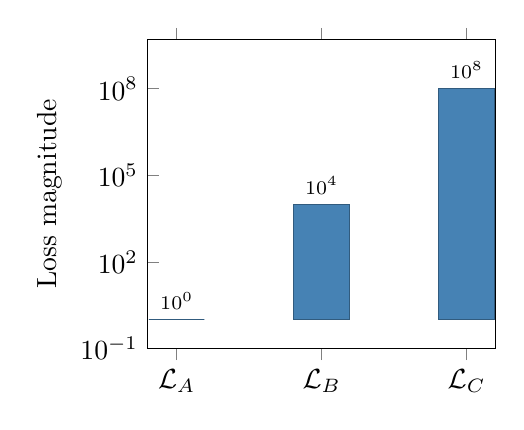
\begin{tikzpicture}
    \begin{axis}[
        ybar,
        width=6cm, height=5.5cm,
        ylabel={Loss magnitude},
        ymode=log,
        symbolic x coords={LA, LB, LC},
        xtick=data,
        xticklabels={$\mathcal{L}_A$, $\mathcal{L}_B$, $\mathcal{L}_C$},
        ymin=0.1, ymax=5e9,
        bar width=20pt,
    ]
    \addplot[fill=softblue, draw=softblue!70!black] coordinates {
        (LA, 1) (LB, 10000) (LC, 100000000)
    };
    \node[font=\scriptsize, above] at (axis cs:LA,1) {$10^{0}$};
    \node[font=\scriptsize, above] at (axis cs:LB,10000) {$10^{4}$};
    \node[font=\scriptsize, above] at (axis cs:LC,100000000) {$10^{8}$};
    \end{axis}
\end{tikzpicture}
\end{center}
\end{columns}
\end{frame}

% --- Slide 4: Multi-Output Network ---
\begin{frame}{One Network, Several Equilibrium Conditions}
\begin{center}
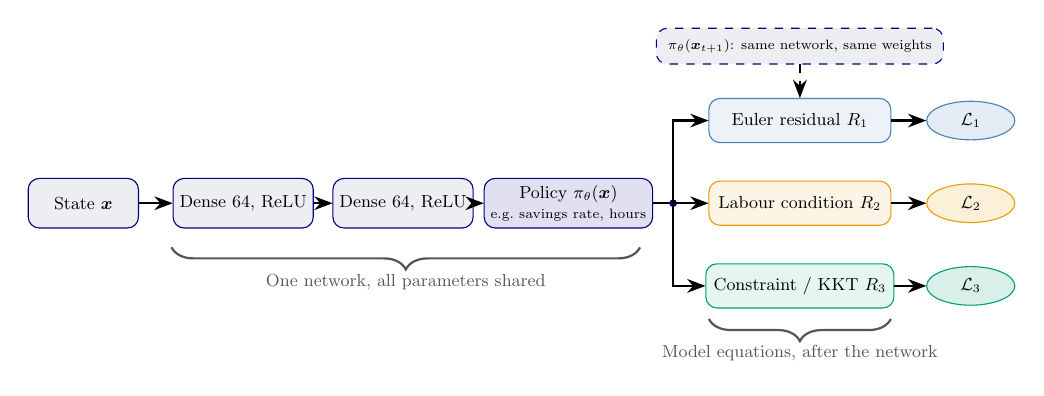
\begin{tikzpicture}[scale=0.70, transform shape,
    block/.style={rectangle, draw=uzhblue, fill=uzhgreylight, rounded corners,
                  minimum height=0.9cm, minimum width=2cm, align=center, font=\small},
    resbase/.style={rectangle, rounded corners, minimum height=0.8cm,
                    minimum width=3.3cm, inner xsep=4pt, align=center, font=\small},
    lossbase/.style={ellipse, minimum height=0.7cm, minimum width=1.6cm,
                     align=center, font=\small},
    >=Stealth,
]
    % Input
    \node[block] (input) at (0,0) {State $\x$};

    % One network: trunk and one output layer
    \node[block, minimum width=2.5cm] (h1) at (2.9,0) {Dense 64, ReLU};
    \node[block, minimum width=2.5cm] (h2) at (5.8,0) {Dense 64, ReLU};
    \node[block, minimum width=2.6cm, fill=uzhblue!12] (pol) at (8.8,0) {Policy $\pi_\theta(\x)$\\[-1pt]{\scriptsize e.g.\ savings rate, hours}};

    % Residuals: each one uses every output
    \node[resbase, draw=softblue, fill=softblue!10] (rA) at (13.0, 1.5) {Euler residual $R_1$};
    \node[resbase, draw=softorange, fill=softorange!10] (rB) at (13.0, 0) {Labour condition $R_2$};
    \node[resbase, draw=softgreen, fill=softgreen!10] (rC) at (13.0,-1.5) {Constraint / KKT $R_3$};

    % The same network at next period's state, needed by the Euler equation
    \node[block, dashed, minimum width=0pt, minimum height=0.65cm, inner xsep=6pt, font=\scriptsize] (next) at (13.0,2.85)
          {$\pi_\theta(\x_{t+1})$: same network, same weights};

    % Losses
    \node[lossbase, draw=softblue, fill=softblue!15] (lossA) at (16.1, 1.5) {$\mathcal{L}_1$};
    \node[lossbase, draw=softorange, fill=softorange!15] (lossB) at (16.1, 0) {$\mathcal{L}_2$};
    \node[lossbase, draw=softgreen, fill=softgreen!15] (lossC) at (16.1,-1.5) {$\mathcal{L}_3$};

    % Arrows: the whole policy fans out to every residual from one junction
    \coordinate (j) at (10.7,0);
    \draw[->, thick] (input) -- (h1);
    \draw[->, thick] (h1) -- (h2);
    \draw[->, thick] (h2) -- (pol);
    \draw[thick] (pol.east) -- (j);
    \fill[uzhblue] (j) circle (2pt);
    \draw[->, thick] (j) |- (rA.west);
    \draw[->, thick] (j) -- (rB.west);
    \draw[->, thick] (j) |- (rC.west);
    \draw[->, thick, dashed] (next.south) -- (rA.north);
    \draw[->, thick] (rA) -- (lossA);
    \draw[->, thick] (rB) -- (lossB);
    \draw[->, thick] (rC) -- (lossC);

    % Braces
    \draw[decorate, decoration={brace, amplitude=8pt, mirror},
          uzhgreydark, thick] (1.6,-0.8) -- (10.1,-0.8)
          node[midway, below=10pt, font=\small] {One network, all parameters shared};
    \draw[decorate, decoration={brace, amplitude=8pt, mirror},
          uzhgreydark, thick] (11.35,-2.1) -- (14.65,-2.1)
          node[midway, below=10pt, font=\small] {Model equations, after the network};
\end{tikzpicture}
\end{center}

\vspace{-0.15cm}
\[
    \mathcal{L}_\text{total} = w_1 \mathcal{L}_1 + w_2 \mathcal{L}_2 + w_3 \mathcal{L}_3,
    \qquad \mathcal{L}_k = \mathbb{E}_{\x}\!\left[R_k(\x;\theta)^2\right]
\]
\vspace{-0.35cm}

{\small The components are equations, not outputs: every residual reads the whole policy, no head owns a loss,
and every parameter receives the sum of all three gradients.}
\emphc{How should we set $w_1, w_2, w_3$?}
\end{frame}

% ============================================================================
% PART 2: LOSS BALANCING STRATEGIES
% ============================================================================

% --- Slide 5: Section Divider ---
{\setbeamercolor{background canvas}{bg=uzhblue}
\setbeamercolor{normal text}{fg=white}
\usebeamercolor[fg]{normal text}
\begin{frame}[plain,c]
\begin{center}
{\Huge\bfseries Loss Balancing Strategies}
\end{center}
\end{frame}
}

% --- Slide 6: Equal Weighting ---
\begin{frame}{Equal Weighting}
\begin{columns}[T]
\column{0.52\textwidth}
\textbf{Simplest approach:} $w_A = w_B = w_C = 1$
\[
    \mathcal{L} = \mathcal{L}_A + \mathcal{L}_B + \mathcal{L}_C
\]

\vspace{0.2cm}
\textbf{Problem:}
\begin{itemize}
    \item If $\mathcal{L}_C \gg \mathcal{L}_A$, gradients are \emphc{dominated} by $\mathcal{L}_C$
    \item Network learns to minimize $\mathcal{L}_C$ first
    \item $\mathcal{L}_A$ barely decreases
    \item Small-scale structure is \emph{ignored}
\end{itemize}

\column{0.45\textwidth}
\begin{block}{Gradient dominance}
\[
    \frac{\partial \mathcal{L}}{\partial \bm{\theta}} \approx \frac{\partial \mathcal{L}_C}{\partial \bm{\theta}}
    \quad\text{when } \mathcal{L}_C \gg \mathcal{L}_A, \mathcal{L}_B.
\]

The network effectively solves a \emph{single-task} problem.
\end{block}
\end{columns}
\end{frame}

% --- Slide 7: Equal Weighting Failure ---
\begin{frame}{Equal Weighting: Training Dynamics}
\begin{center}
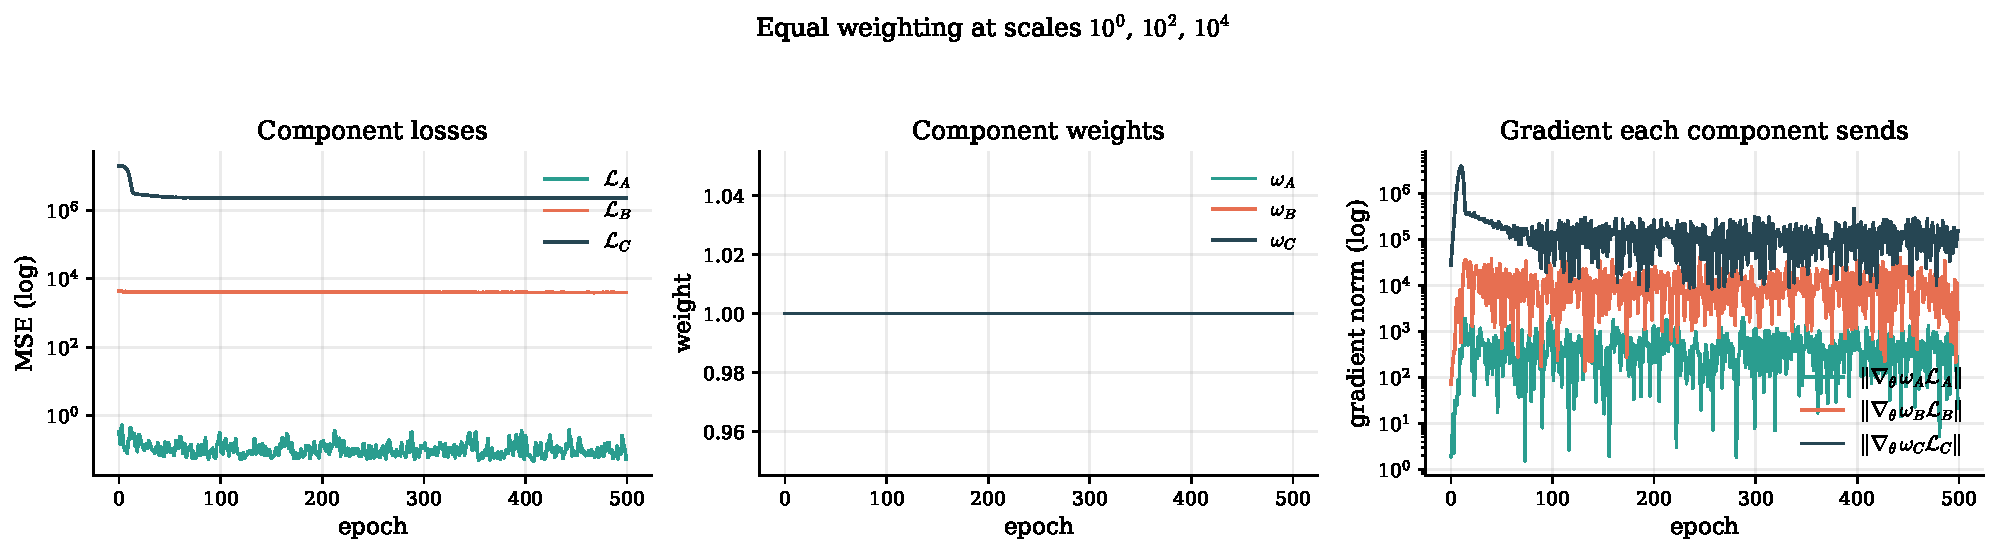
\includegraphics[width=0.95\linewidth]{figures/loss_norm_equal_weights.pdf}
\end{center}

\vspace{-0.3em}
{\footnotesize Stored teaching run of \texttt{03\_03}, Section 3. Left: component MSE on a log axis. Middle: the constant weights. Right, the panel to read: the norm of the gradient each component sends to the shared parameters, $2.2\cdot10^{1}$, $1.9\cdot10^{3}$, $1.6\cdot10^{5}$ at the end. The update is their sum, so the trunk serves $f_C$ and the other two get what is left. Which of them ends up worst is not the smaller one by default: here it is $f_B$, at 54\% relative error, against 18\% for $f_A$.}
\end{frame}

% --- Slide 7b: Fix 0, natural units ---
\begin{frame}{Fix 0: Write Each Residual in Its Natural Units}
\small
Every equilibrium residual has a scale of its own: a consumption, an output, a marginal utility.
Dividing the residual by that scale \emphc{before} it enters the loss costs nothing, adds no
hyperparameter, and removes the problem at the source.

\vspace{0.15cm}
\begin{columns}[T]
\column{0.52\textwidth}
\textbf{As coded in Session 5 (\texttt{05\_01}, \texttt{05\_02}):}
\begin{itemize}\itemsep2pt
  \item Euler equation: divided by $\lambda_t$, so the residual is relative to the marginal value of resources
  \item Resource constraint: divided by total resources $\sum_j [Y_t^j + (1-\delta)k_t^j]$
  \item Complementarity: Fischer--Burmeister on the unit-free pair $(\mu_t^j/\lambda_t,\; I_t^j/k_t^j)$
\end{itemize}
Then the three components are weighted \textbf{equally}.
\column{0.45\textwidth}
\textbf{On the toy problem} (\texttt{03\_03}, Section 4):
\begin{center}
\renewcommand{\arraystretch}{1.15}
{\scriptsize
\begin{tabular}{@{}lr@{}}
\toprule
 & total rel.\ error \\
\midrule
equal weights, scales $1, 10^2, 10^4$ & 0.861 \\
residuals divided by their scale & 0.011 \\
\bottomrule
\end{tabular}}
\end{center}
{\scriptsize A factor 75$\times$ from a change of units. Every adaptive rule in this deck is judged against this line.}
\end{columns}
\end{frame}

% --- Slide 8: Manual Weighting ---
\begin{frame}{Manual Weighting}
\small
\vspace{-0.1cm}
\textbf{Idea:} Choose weights to approximately equalize the loss magnitudes:
\[
    \mathcal{L} = w_A \cdot \mathcal{L}_A + w_B \cdot \mathcal{L}_B + w_C \cdot \mathcal{L}_C
\]
e.g., $w_A = 10^4,\; w_B = 10^0,\; w_C = 10^{-2}$.

\vspace{0.3cm}
\begin{columns}[T]
\column{0.48\textwidth}
\textbf{Pros:}
\begin{itemize}
    \item Can work well if scales are known a priori
    \item Simple to implement
\end{itemize}

\column{0.48\textwidth}
\textbf{Cons:}
\begin{itemize}
    \item \emphc{Trial-and-error}: need to tune $d$ extra hyperparameters
    \item \emphc{Fragile}: optimal weights change during training as losses evolve
    \item \emphc{Doesn't generalize}: weights are problem-specific
\end{itemize}
\end{columns}

\vspace{0.2cm}
\begin{alertblock}{Natural units first; then, for what remains, a rule that adapts during training.}
\end{alertblock}
\end{frame}

% --- Slide 9: Inverse-Loss Weighting ---
\begin{frame}{Inverse-Loss Weighting}
\begin{columns}[T]
\column{0.55\textwidth}
\textbf{Idea:} Weight each component inversely proportional to its current magnitude:
\[
    w_i^{(t)} = \frac{1}{\mathcal{L}_i^{(t)}}
\]

This automatically up-weights small losses and down-weights large ones.

\vspace{0.3cm}
\textbf{With exponential averaging} (for stability):
\[
    \bar{\mathcal{L}}_i^{(t)} = \beta_{\mathrm{ema}} \cdot \bar{\mathcal{L}}_i^{(t-1)} + (1 - \beta_{\mathrm{ema}}) \cdot \mathcal{L}_i^{(t)}
\]
\[
    w_i^{(t)} = \frac{1}{\bar{\mathcal{L}}_i^{(t)} + \epsilon}
\]

\column{0.42\textwidth}
\textbf{Pros:}
\begin{itemize}
    \item Simple, one hyperparameter ($\beta_{\mathrm{ema}}$)
    \item Adapts to scales it does not know in advance
\end{itemize}

\vspace{0.3cm}
\textbf{Cons:}
\begin{itemize}
    \item It equalizes the \emph{weighted losses} $w_i\mathcal{L}_i$, not the gradients
    \item The gradient of $w_i\mathcal{L}_i$ then scales like $1/e_i$: the component fit \emphc{best} pushes hardest
    \item Unstable as $\mathcal{L}_i \to 0$
\end{itemize}
\end{columns}
\end{frame}

% --- Slide 10: Inverse-loss, what it does to the gradients ---
\begin{frame}{Inverse-Loss Weighting: The Gradients}
\begin{center}
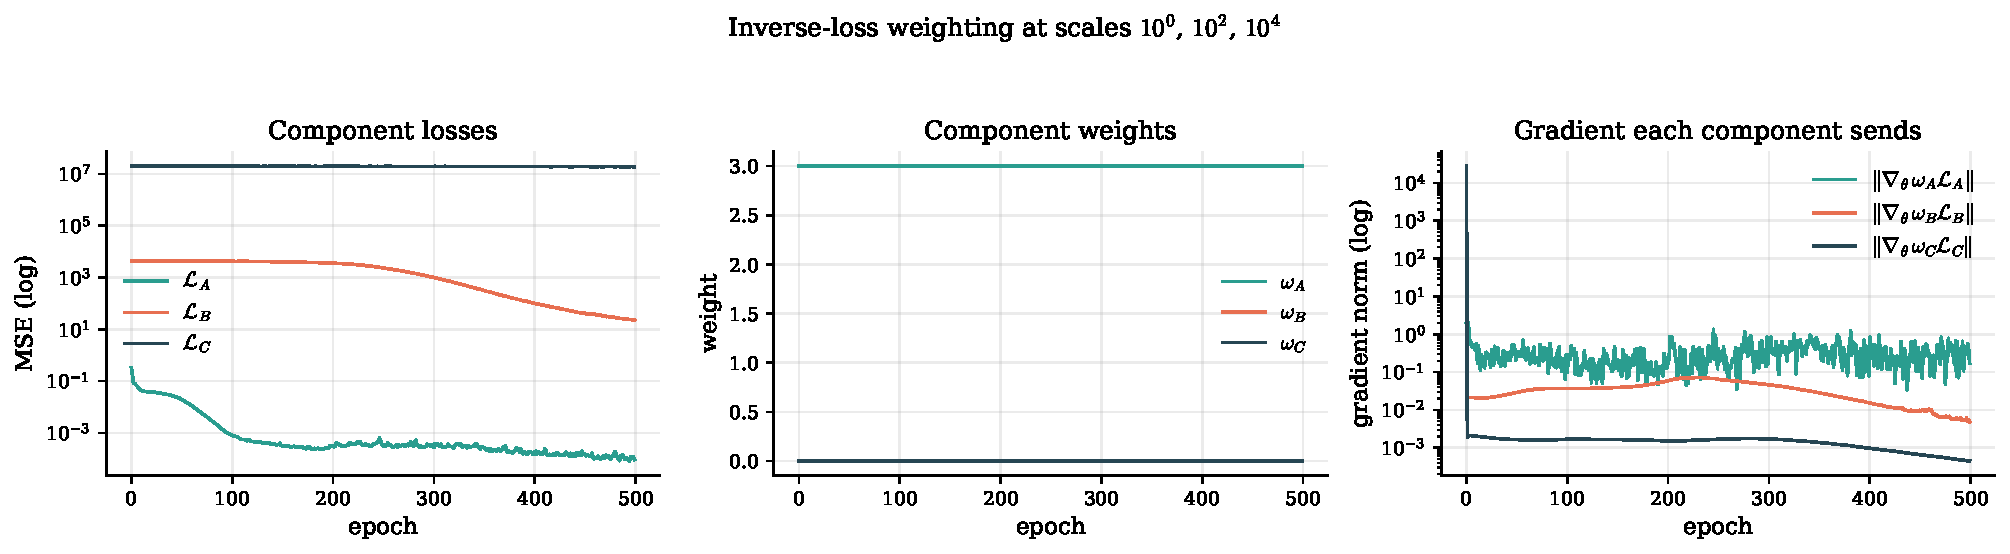
\includegraphics[width=0.95\linewidth]{figures/loss_norm_inverse_weights.pdf}
\end{center}

\vspace{-0.3em}
{\footnotesize Stored teaching run of \texttt{03\_03}, Section 5, $\beta_{\mathrm{ema}} = 0.99$, weights normalized to $\sum_i w_i = 3$. The weights end $7.0\cdot10^{9}$$\times$ apart and the weighted losses are equal, as designed. The right panel shows the consequence: the gradient goes to whichever component is currently best fit. Total relative error 0.448 against 0.861 for equal weights and 0.011 for natural units.}
\end{frame}

% --- Slide 11: SoftAdapt ---
\begin{frame}{SoftAdapt}
\small
\textbf{Idea} (Heydari et al., 2019): weight by \emph{relative loss change}. A component whose loss is rising, or falling slowly, gets more weight; $T$ sets how sharply.

\vspace{0.1cm}
\begin{block}{Weight update}
\vspace{-0.15cm}
\[
    \hat{w}_i^{(t)} = K \, \frac{\exp\!\bigl(\Delta_i^{(t)} / T\bigr)}{\sum_{j} \exp\!\bigl(\Delta_j^{(t)} / T\bigr)},
    \qquad \Delta_i^{(t)} = \mathcal{L}_i^{(t)} - \mathcal{L}_i^{(t-1)}
\]
\end{block}

\vspace{0.1cm}
\begin{columns}[T]
\column{0.48\textwidth}
\textbf{Pros:} focuses on the \emph{struggling} component; a few lines of code.
\column{0.48\textwidth}
\textbf{Cons:} sensitive to $T$; noisy loss changes give noisy weights. Not in the notebook; ReLoBRaLo is its successor.
\end{columns}

\vspace{0.15cm}
\begin{alertblock}{Scale caveat}
\footnotesize
Raw $\Delta_i$ carries the units of $\mathcal{L}_i$: a component at $10^{8}$ swamps one at $10^{0}$ inside the softmax. Rescale, $\tilde\Delta_i = \Delta_i / (\mathcal{L}_i + \varepsilon)$, so the rule reacts to \emph{relative} progress. ReLoBRaLo builds that in.
\end{alertblock}
\end{frame}

% --- Slide 13: ReLoBRaLo Idea ---
\begin{frame}{ReLoBRaLo: Relative Loss Balancing with Random Lookback}
\begin{columns}[T]
\column{0.55\textwidth}
\textbf{Key ingredients} (Bischof \& Kraus, 2021; CMAME 2025), adapted here as a deterministic classroom version:

\vspace{0.2cm}
\begin{enumerate}
    \item \textbf{Relative balancing:} Use \emph{ratios} $\mathcal{L}_i^{(t)} / \mathcal{L}_i^{(t-1)}$ instead of absolute values

    \vspace{0.2cm}
    \item \textbf{Baseline comparison:} Mix in the \emphc{initial losses} $\mathcal{L}_i^{(0)}$ as a stable reference

    \vspace{0.2cm}
    \item \textbf{Exponential smoothing:} Blend new weights with history via $\alpha$
\end{enumerate}

\column{0.42\textwidth}
\begin{block}{Why a lookback at all?}
Step ratios $\mathcal{L}_i^{(t)}/\mathcal{L}_i^{(t-1)}$ sit near $1$ for every component and say nothing about how far each has come. With probability $\rho$ the update compares with the previous step, otherwise with the \emph{initial} loss, so the weights stay anchored to the starting point. The classroom version blends the two deterministically with weight $\rho$.
\end{block}
\end{columns}
\end{frame}

% --- Slide 14: ReLoBRaLo Algorithm ---
\begin{frame}{ReLoBRaLo: Algorithm}
\begin{block}{Weight update at epoch $t$}
\begin{algorithmic}[1]
\STATE Compute losses $\mathcal{L}_1^{(t)}, \ldots, \mathcal{L}_K^{(t)}$
\STATE \textbf{Step-wise ratios:}\; $r_{i,s}^{(t)}=\mathcal{L}_i^{(t)}/(T\mathcal{L}_i^{(t-1)}+\varepsilon)$
\STATE \textbf{Baseline ratios:}\; $r_{i,b}^{(t)}=\mathcal{L}_i^{(t)}/(T\mathcal{L}_i^{(0)}+\varepsilon)$
\STATE $\hat w_{i,s}^{(t)}=K\,\operatorname{softmax}_i(r_{\cdot,s}^{(t)})$,\quad
       $\hat w_{i,b}^{(t)}=K\,\operatorname{softmax}_i(r_{\cdot,b}^{(t)})$
    \STATE \textbf{Combine with smoothing:}
\[
    w_i^{(t)} = \alpha \Bigl[\rho \, w_i^{(t-1)} + (1-\rho) \, \hat{w}_{i,b}^{(t)}\Bigr]
    + (1-\alpha) \, \hat{w}_{i,s}^{(t)}
\]
\end{algorithmic}
\end{block}

\vspace{0.3cm}
\begin{itemize}
    \item $\alpha$: smoothing, how much to trust the historical weights
    \item $\rho$: baseline mix, relative weight on the initial-loss comparison
    \item $T$: temperature, sharpness of the softmax
\end{itemize}
\end{frame}

% --- Finger Exercise: ReLoBRaLo ---
\begin{frame}{\exercisepause{} Finger Exercise: Loss Balancing}
\begin{exampleblock}{Exercise}
A DEQN has three loss components at iteration $t$: $\mathcal{L}_1^{(t)} = 10.0$, $\mathcal{L}_2^{(t)} = 0.01$, $\mathcal{L}_3^{(t)} = 1.0$.
\begin{enumerate}
    \item If you use \emphc{equal weights} $w_i = 1/3$, which loss component dominates the gradient? Is this desirable?
    \item Compute the \emphc{inverse-loss weights}: $w_i \propto 1/\mathcal{L}_i^{(t)}$, normalized to sum to 1.
    \item Which component now receives the highest weight? Why does this help training?
\end{enumerate}
\end{exampleblock}
\end{frame}

\begin{frame}{Solution: Loss Balancing}
\begin{block}{Answer}
\begin{enumerate}
    \item With equal weights, $\mathcal{L}_1 = 10.0$ dominates (100$\times$ larger than $\mathcal{L}_2$). The optimizer focuses almost entirely on reducing $\mathcal{L}_1$ while ignoring $\mathcal{L}_2$. This is undesirable if all three conditions must be satisfied simultaneously.
    \item Unnormalized: $1/10.0 = 0.1$, $1/0.01 = 100$, $1/1.0 = 1$. Sum = 101.1.\\
    Normalized: $w_1 = 0.001$, $w_2 = 0.989$, $w_3 = 0.010$.
    \item $\mathcal{L}_2$ receives the highest weight ($\approx 99\%$), and the three weighted losses are now equal at $\approx 0.01$. That is the whole content of the rule: it equalizes levels. Whether that is what training needs is a different question; the notebook (Section 5) shows the gradient then flows to the component that is currently fit best.
\end{enumerate}
\end{block}
\end{frame}

% --- Slide 15: ReLoBRaLo Hyperparameters ---
\begin{frame}{ReLoBRaLo: Hyperparameters}
\small
\begin{center}
\vspace{-0.2cm}
\footnotesize
\renewcommand{\arraystretch}{1.2}
\begin{tabular}{@{}c l c p{6.2cm}@{}}
\toprule
\textbf{Symbol} & \textbf{Name} & \textbf{Default} & \textbf{Effect} \\
\midrule
$T$      & Temperature   & $1.0$   & Softmax sharpness: small $T$ $\to$ winner-take-all; large $T$ $\to$ uniform weights. \\
$\alpha$ & Smoothing     & $0.999$ & Each update moves the weight $0.1\%$ of the way to its target: a time constant of about $1000$ \emph{updates}. \\
$\rho$   & Baseline mix  & $0.999$ & Weight on the initial-loss comparison (convex blend here, Bernoulli in the original). \\
\bottomrule
\end{tabular}
\end{center}

\vspace{0.25cm}
{\footnotesize \emphc{Two ceilings.} The softmax separates two weights by at most $e^{\Delta\kappa/T}$ per update, about $e$ at $T=1$; the smoothing needs about $1/(1-\alpha)$ updates to get there. Per \emph{epoch}, 500 updates, the weights barely move at any $T$; per \emph{optimizer step}, as the authors do, they can. \texttt{03\_03} runs both.}

\vspace{0.15cm}
\begin{block}{Practical guidance}
Update per step, not per epoch. Non-dimensionalize first; then $T$ hardly matters.
\end{block}
\end{frame}

% --- Slide 16: ReLoBRaLo Visual ---
\begin{frame}{ReLoBRaLo: Weight Evolution}
\begin{center}
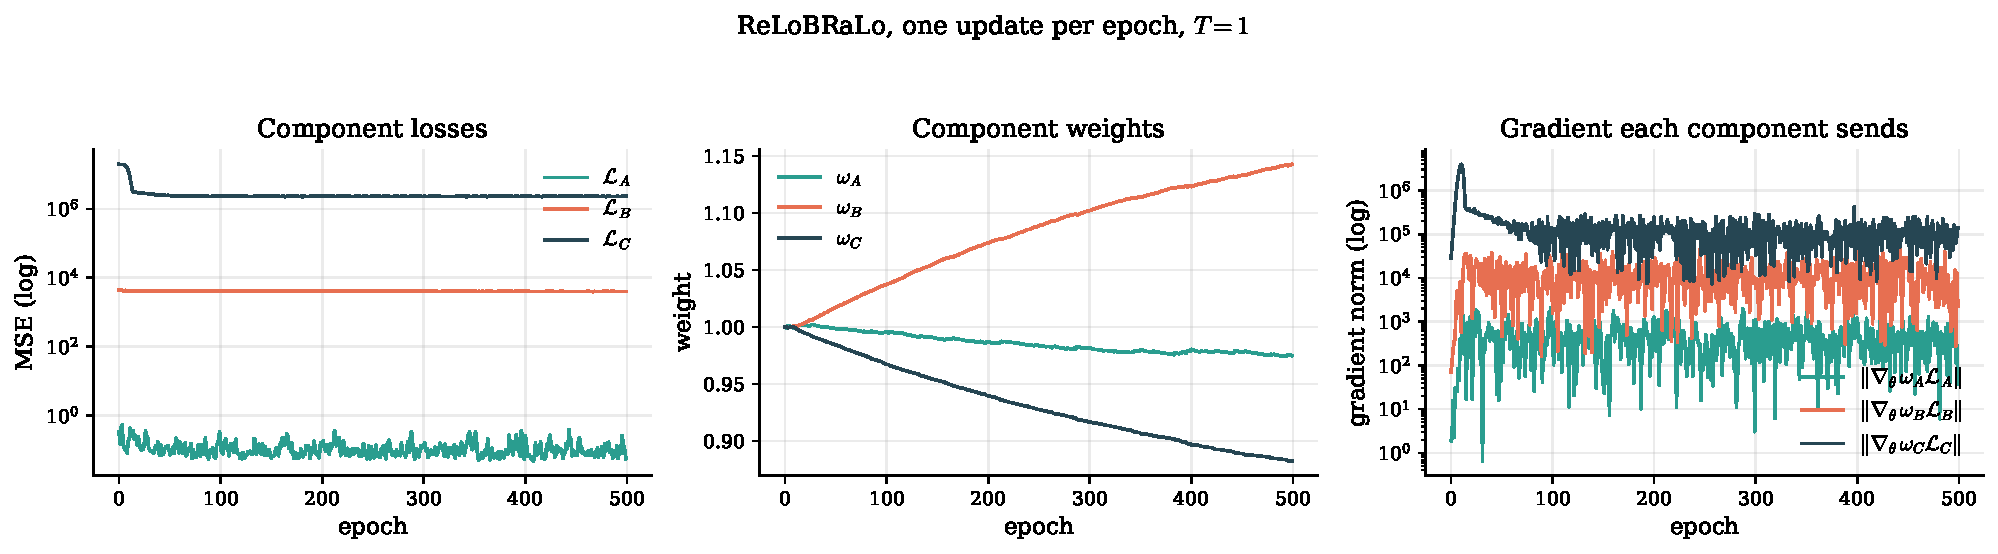
\includegraphics[width=0.95\linewidth]{figures/loss_norm_relobralo_weights.pdf}
\end{center}

\vspace{-0.3em}
{\footnotesize Stored teaching run of \texttt{03\_03}, Section 6, one update per epoch, $T=1$. The weights move by 1.29$\times$ in 500 updates, and the loss and gradient panels are indistinguishable from equal weighting: total relative error 0.861 against 0.861. Per optimizer step (7,500 updates) the weights reach 1.5$\times$ and the total is 0.871. Per step the rule has the authority it was designed with, and it still lands at 0.871, 76$\times$ above natural units: relative balancing is not what a gap in the units needs.}
\end{frame}

% --- Slide 17: GradNorm ---
\begin{frame}{GradNorm: Balance the Gradients Themselves}
\small
\textbf{Idea} (Chen et al., 2018): equalize the quantity in the right-hand panels of the last three figures, the gradient norm each weighted component sends to the shared parameters.

\vspace{0.05cm}
\begin{block}{Gradient-balance loss}
\vspace{-0.15cm}
\[
    \mathcal{L}_\text{grad} = \sum_{i=1}^{K} \Bigl| \bigl\| \nabla_{\bm{\theta}}\, w_i \mathcal{L}_i \bigr\|_2 - \bar{G}\, r_i^{(t)} \Bigr|,
    \qquad r_i^{(t)} = \Bigl(\tilde{\mathcal{L}}_i^{(t)} \big/ \text{mean}_j\, \tilde{\mathcal{L}}_j^{(t)}\Bigr)^{\alpha},
    \quad \tilde{\mathcal{L}}_i^{(t)} = \mathcal{L}_i^{(t)}/\mathcal{L}_i^{(0)}
\]
\end{block}
$\bar G$ is the mean gradient norm; $r_i$ raises the target for the component with the least relative progress ($\alpha = 1.5$ typical). The $w_i$ are trained by gradient descent on $\mathcal{L}_\text{grad}$ and renormalized to $\sum_i w_i = K$.

\vspace{0.05cm}
\begin{columns}[T]
\column{0.48\textwidth}
\textbf{Pros:} acts on the gradient, which is what dominance is; can balance a permanent scale gap in principle.
\column{0.48\textwidth}
\textbf{Cons:} one extra backward pass per component per update; a second optimizer with its own learning rate and $\alpha$.
\end{columns}

\vspace{0.05cm}
{\scriptsize Cheaper cousin for PINNs: Wang, Teng \& Perdikaris (2021) set $w_i$ from the ratio of gradient norms directly.}
\end{frame}

% ============================================================================
% PART 3: EXPERIMENT
% ============================================================================

% --- Slide 19: Section Divider ---
{\setbeamercolor{background canvas}{bg=uzhblue}
\setbeamercolor{normal text}{fg=white}
\usebeamercolor[fg]{normal text}
\begin{frame}[plain,c]
\begin{center}
{\Huge\bfseries Experiment: Multi-Scale}\\[0.3cm]
{\Large\bfseries Function Approximation}
\end{center}
\end{frame}
}

% --- Slide 20: Setup ---
\begin{frame}{Experiment Setup}
\begin{columns}[T]
\column{0.50\textwidth}
\textbf{Three target functions} on $[0,1]^2$:

\vspace{0.2cm}
\begin{tabular}{@{}lrl@{}}
$f_A(\x)$ & $=$ & $\text{genz\_gaussian}(\x)$ \\
           &     & scale $\in [0, 1]$ \\[4pt]
$f_B(\x)$ & $=$ & $100 \times \text{genz\_oscillatory}(\x)$ \\
           &     & scale $\in [-100, 100]$ \\[4pt]
$f_C(\x)$ & $=$ & $10{,}000 \times \text{genz\_continuous}(\x)$ \\
           &     & scale $\in [0, 10{,}000]$ \\
\end{tabular}

\column{0.47\textwidth}
\textbf{Architecture:}
\begin{itemize}
    \item Shared trunk: $3 \times 64$ ReLU
    \item 3 output heads (Dense(1) each)
    \item Adam, $\eta = 10^{-3}$
\end{itemize}

{\small The heads stand in for residuals; what the testbed shares with a DEQN is the trunk.}

\vspace{0.2cm}
\textbf{Data and budget:}
\begin{itemize}
    \item $n_\text{train} = 1{,}000$, $n_\text{test} = 2{,}000$, $d = 2$
    \item 500 epochs, batch 64; three seeds per rule
\end{itemize}
\end{columns}

\vspace{0.3cm}
\[
    \mathcal{L} = w_A \cdot \text{MSE}(f_A, \hat{f}_A) + w_B \cdot \text{MSE}(f_B, \hat{f}_B) + w_C \cdot \text{MSE}(f_C, \hat{f}_C)
\]
\end{frame}

% --- Slide 21: Results ---
\begin{frame}{Results: Every Rule Against Natural Units}
\footnotesize
\vspace{-0.1cm}
\begin{center}
\renewcommand{\arraystretch}{0.95}
\setlength{\tabcolsep}{4pt}
{\footnotesize
\begin{tabular}{@{}lccccc@{}}
\toprule
 & \textbf{Equal} & \textbf{Inverse-loss} & \textbf{ReLoBRaLo} & \textbf{ReLoBRaLo} & \textbf{Natural units} \\
 & & & per epoch & per step & (equal weights) \\
\midrule
rel.\ error $f_A$, seed 0 & 0.177 & 0.0082 & 0.177 & 0.177 & 0.0030 \\
rel.\ error $f_B$, seed 0 & 0.540 & 0.033 & 0.539 & 0.539 & 0.0022 \\
rel.\ error $f_C$, seed 0 & 0.116 & 0.407 & 0.116 & 0.116 & 0.0031 \\
\midrule
total, median of 3 seeds & 0.861 & 0.448 & 0.861 & 0.871 & \emphc{0.011} \\
range & 0.833--0.924 & 0.418--0.609 & 0.833--0.933 & 0.832--0.931 & 0.0083--0.018 \\
\bottomrule
\end{tabular}
}
\end{center}

\vspace{0.15cm}
\begin{itemize}\itemsep0pt
    \item \textbf{Equal:} $f_C$ owns the gradient; the total relative error is 0.861.
    \item \textbf{Inverse-loss:} equalizes the weighted losses; total 0.448, the gradient goes to the best-fit component and $f_C$ pays (0.407 against 0.116).
    \item \textbf{ReLoBRaLo:} per epoch, identical to equal weighting, the smoothing never lets the weights move. Per step, the weights spread 1.5$\times$ and the total is 0.871: no better.
    \item \textbf{Natural units:} 0.011, a factor 75 below equal weighting, from a change of units.
\end{itemize}

{\scriptsize Stored teaching run of \texttt{03\_03}, 500 epochs, seeds 0, 1, 2. Relative error $= \overline{|e_i|}/\text{scale}_i$ on 2,000 test points; total is the sum over the three components.}
\end{frame}

% --- Slide 23: Sensitivity to T ---
\begin{frame}{Sensitivity to Temperature $T$}
\begin{columns}[T]
\column{0.55\textwidth}
\begin{center}
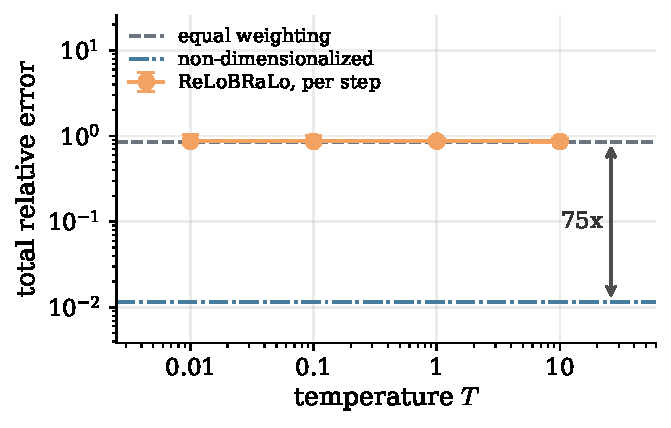
\includegraphics[width=\linewidth, height=3.3cm, keepaspectratio]{figures/loss_norm_T_sensitivity.pdf}
\end{center}
\vspace{-0.2cm}
{\scriptsize ReLoBRaLo per step, three seeds per $T$: median and range of the total relative error (\texttt{03\_03}, Section 7).}

\column{0.42\textwidth}
\vspace{0.1cm}
\textbf{$T$ small ($\ll 1$):}
\begin{itemize}\itemsep0pt
    \item Winner-take-all softmax
    \item Weights can separate far, if the smoothing lets them
\end{itemize}

\vspace{0.15cm}
\textbf{$T$ large ($\gg 1$):}
\begin{itemize}\itemsep0pt
    \item Near-equal weights
    \item Reverts to the scale problem
\end{itemize}

\vspace{0.05cm}
\textbf{Measured:} medians from 0.863 ($T=10$) to 0.871 ($T=1$); the final weight spread runs from 1.0$\times$ to 4$\times$.
\end{columns}

\vspace{0.15cm}
{\small The gap to natural units is 75$\times$ or more at every temperature: $T$ is not the lever for a scale gap that sits in the units.}
\end{frame}

% --- Slide 23b: the same measurement on a DEQN ---
\begin{frame}{The Same Measurement on a DEQN}
\footnotesize
Brock--Mirman with endogenous labour (\texttt{02\_04}, Exercise 2): two policies, two first-order
conditions, each in \emph{levels} or in \emph{relative} form. Same $2\times64$ network, states,
optimizer, seed, 3{,}000 episodes; the gradient norm of each condition recorded every episode.

\vspace{-0.05cm}
\begin{center}
\renewcommand{\arraystretch}{0.95}
{\scriptsize
\begin{tabular}{@{}ll rrr rr@{}}
\toprule
 & & \multicolumn{3}{c}{gradient-norm ratio, labour / Euler} & \multicolumn{2}{c}{final mean $|$rel.\ error$|$} \\
form & weights & episode 1 & episode 300 & last & Euler & labour \\
\midrule
levels   & equal        & $2.6\cdot10^{1}$ & $3.9\cdot10^{0}$ & $3.0\cdot10^{0}$ & $2.6\cdot10^{-2}$ & $1.1\cdot10^{-2}$ \\
relative & equal        & $1.2\cdot10^{5}$ & $3.6\cdot10^{0}$ & $1.0\cdot10^{0}$ & $2.9\cdot10^{-2}$ & $6.3\cdot10^{-3}$ \\
levels   & inverse-loss & $2.6\cdot10^{1}$ & $1.2\cdot10^{0}$ & $7.4\cdot10^{1}$ & $2.5\cdot10^{-2}$ & $2.1\cdot10^{-3}$ \\
relative & inverse-loss & $1.2\cdot10^{5}$ & $2.7\cdot10^{-1}$ & $1.4\cdot10^{0}$ & $3.4\cdot10^{-3}$ & $1.2\cdot10^{-1}$ \\
\bottomrule
\end{tabular}}
\end{center}

\vspace{0.1cm}
\begin{itemize}\itemsep0pt\scriptsize
  \item A random initial policy violates the labour condition far more than the Euler equation: a gradient-norm gap of $1.2\cdot10^{5}$ at episode 1 in relative form. It is \emphc{transient}: the intratemporal condition is easy, and by episode 300 the two send gradients of the same order. Equal weights survive it.
  \item Inverse-loss weighting shortens the transient and then keeps acting: in levels the labour error improves to $2.1\cdot10^{-3}$ from $1.1\cdot10^{-2}$; in relative form the small labour loss gets a near-zero weight and the labour error drifts to $1.2\cdot10^{-1}$ from $6.3\cdot10^{-3}$. A rule that balances levels cannot tell a solved condition from a neglected one.
  \item The Genz gap never closes because it is in the units. Same diagnostic in both cases: the ratio \emph{after} the transient. {\scriptsize (Stored teaching run of \texttt{03\_03}, Section 8.)}
\end{itemize}
\end{frame}

% --- Slide 24: Connection to PINNs and DSGE ---
\begin{frame}{Connection to PINNs and DSGE}
\small
\begin{columns}[T]
\column{0.50\textwidth}
\textbf{Physics-informed NNs:}
\begin{itemize}
    \item PDE residual: $\mathcal{L}_\text{PDE} \sim \mathcal{O}(1)$
    \item Boundary conditions: $\mathcal{L}_\text{BC} \sim \mathcal{O}(10^{-2})$
    \item Initial conditions: $\mathcal{L}_\text{IC} \sim \mathcal{O}(10^{-4})$
    \item Rate-balancing rules keep BCs/ICs from being \emphc{ignored} once the units agree
\end{itemize}

\column{0.47\textwidth}
\textbf{DSGE / Deep equilibrium nets:}
\begin{itemize}
    \item Euler equations, one per agent or country
    \item Budget and resource constraints, in goods units
    \item Complementarity conditions, in multiplier units
    \item Session 5 divides each by its own scale, then weights equally
\end{itemize}
\end{columns}

\vspace{0.1cm}
\begin{block}{Where the adaptive rules belong}
Bischof \& Kraus apply ReLoBRaLo to PINN losses that are already non-dimensionalized, to balance components that converge at different rates. That is the case in the right column after the units are fixed, and the case Session 8 returns to.
\end{block}
\end{frame}

% --- Slide 25: Summary ---
\begin{frame}{Summary}
\footnotesize
\vspace{-0.4cm}
\begin{columns}[T]
\column{0.55\textwidth}
\textbf{Key takeaways:}
\begin{enumerate}\itemsep1pt
    \item Gradient dominance is measurable: record $\|\nabla_\theta\, w_i \mathcal{L}_i\|$ per component.
    \item \textbf{Natural units first.} Free, no hyperparameters, two orders of magnitude on the testbed.
    \item Inverse-loss weighting equalizes levels, and sends the gradient to the best-fit component.
    \item ReLoBRaLo balances progress: a ceiling of about $e^{1/T}$, reached only with per-step updates.
    \item A transient gap closes on its own; a permanent one needs different units, not a rule.
\end{enumerate}

\column{0.42\textwidth}
\textbf{References:}
{\scriptsize
\begin{itemize}\itemsep0pt
    \item Bischof \& Kraus (2021). \emph{Multi-Objective Loss Balancing for Physics-Informed Deep Learning}, arXiv:2110.09813; \emph{CMAME} 439, 117914 (2025).
    \item Chen et al.\ (2018). \emph{GradNorm}, ICML.
    \item Heydari et al.\ (2019). \emph{SoftAdapt}, arXiv:1912.12355.
    \item Wang, Teng \& Perdikaris (2021). \emph{Gradient flow pathologies in PINNs}, SIAM J.\ Sci.\ Comput.\ 43(5).
\end{itemize}
}
\end{columns}

\vspace{0.1cm}
\begin{block}{Hands-on}
$\Rightarrow$ \texttt{03\_03\_Loss\_Normalization.ipynb}
\end{block}
\end{frame}

\end{document}
